% 2015 年重庆卷（文史类）第 21 题：椭圆与过右焦点的弦 PQ（依固定扫描页重绘，只画拓扑与标号，不按比例）
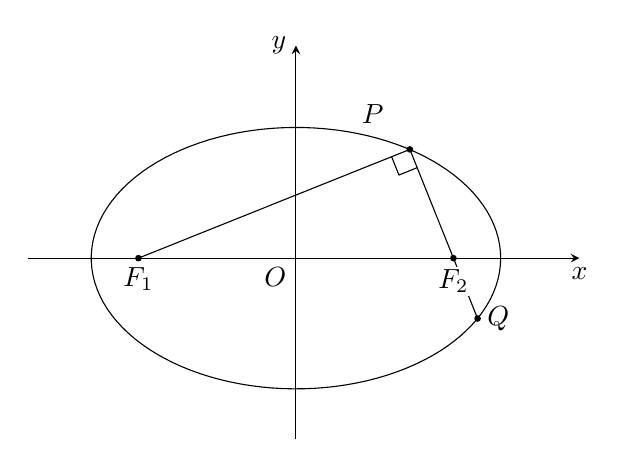
\begin{tikzpicture}[>=stealth,scale=1.0]
  % 坐标轴
  \draw[->] (-3.4,0)--(3.6,0) node[below] {$x$};
  \draw[->] (0,-2.3)--(0,2.7) node[left] {$y$};
  \node[below left] at (0,0) {$O$};
  % 椭圆 x^2/2.6^2 + y^2/1.66^2 = 1
  \draw[domain=0:360,samples=120] plot ({2.6*cos(\x)},{1.66*sin(\x)});
  % 焦点与点
  \coordinate (F1) at (-2,0);
  \coordinate (F2) at (2,0);
  \coordinate (P) at (1.447,1.381);
  \coordinate (Q) at (2.307,-0.767);
  % 弦 PQ 与线段 PF1
  \draw (P)--(Q);
  \draw (P)--(F1);
  % 直角标记（PF1 与 PQ 在 P 处）
  \draw (1.215,1.288)--(1.308,1.056)--(1.540,1.149);
  % 标号
  \fill (F1) circle (1.2pt) node[below] {$F_{1}$};
  \fill (F2) circle (1.2pt) node[fill=white,inner sep=1pt,below=3pt] {$F_{2}$};
  \fill (P) circle (1.2pt) node[above left=6pt] {$P$};
  \fill (Q) circle (1.2pt) node[right] {$Q$};
\end{tikzpicture}
